\chapter{Selección y extracción de variables}

En esta sección se aplicarán diversas técnicas para reducir la cantidad de atributos necesaria para describir cada estrella. Esta reducción se puede alcanzar de dos formas \cite{fs4}:

\begin{itemize}

\item \textbf{Selección de Variables} (Feature Selection): Utilizar un subconjunto de atributos del dataset original, sin transformarlos, por lo tanto manteniendo su interpretación original. Ejemplo: Filtros univariable. (Ver sección \ref{filtros_univ}).
\item \textbf{Extracción de Variables} (Feature Extraction): Transformar los atributos originales en un nuevo conjunto de atributos, reduciendo la cantidad de atributos e intentando conservar la información relevante. Ejemplo: PCA (Ver sección \ref{PCA}).
\end{itemize} 

\section{Selección de variables}
\subsection{Introducción a selección de variables}
\label{seleccion_v}


En la mayoría de los problemas de clasificación con datos provenientes del mundo real, los atributos relevantes son a menudo desconocidos a priori. Usualmente, muchos atributos candidatos son introducidos con el objeto de representar el dominio lo mejor posible. Desafortunadamente, muchos de estos atributos candidatos son parcial o completamente irrelevantes o redundantes para el concepto objetivo \cite{fs2}.  \\ 

Selección de variables, como ya se mencionó, consiste en elegir sólo un subconjunto de atributos de un cierto dataset, descartando los demás de acuerdo a un cierto criterio \cite{fs1}. Realizar selección de variables como un paso previo a aplicar un algoritmo de aprendizaje automatizado puede proveer varias ventajas \cite{fs3}:

\begin{itemize}
\item \textbf{Desempeño}: En ciertos datasets, muchas variables no son informativas para el problema en cuestión. Al eliminar atributos irrelevantes, ruidosos o redundantes, se reduce el riesgo de sobreajuste, mejorando el desempeño del clasificador en test. Más aún, algunos algoritmos simplemente trabajan mucho mejor con menos variables. 
\item \textbf{Eficiencia}: Reducción en complejidad computacional y espacial.
\item \textbf{Entendimiento}: El modelo resulta más sencillo y fácil de interpretar. Adicionalmente, muchas técnicas utilizadas para realizar selección de variables permiten en el proceso descubrir información sobre el problema, por ejemplo cuáles son las variables más importantes (Ver capítulo \ref{inspeccionando}).
\end{itemize}

En este trabajo se aplicaron métodos de selección de variables de \textbf{filtrado} \cite{fs4}, que asignan un puntaje o ranking a atributos individuales o a grupos de atributos. Los \textbf{filtros univariable} asignan un puntaje a cada atributo por separado, mientras que los \textbf{filtros multivariable} evalúan subconjuntos de atributos a la vez. 

\subsection{Filtros univariable}

\label{filtros_univ}

En este trabajo se experimentó únicamente con filtros univariable, los cuales funcionan asignando puntajes a cada atributo intentando medir cuán correlacionado dicho atributo está con la variable a predecir. Posteriormente, se evaluó la performance de nuestro clasificador conservando únicamente los $k$ atributos con mayor puntaje para entrenar y testear. Los filtros utilizados fueron:

\begin{itemize}
\item \textbf{f\_classif}: Computa el ANOVA (Analysis of Variance) F-value \cite{han2012mining}. Este test estadístico determina si las medias de dos muestras de datos provienen de la misma distribución o no. Este test es capaz de medir correlaciones lineares. En la sección \ref{f_test} se estudiará ANOVA en mayor detalle.

\item \textbf{mutual\_info}: Calcula la información mútua  \cite{han2012mining} entre dos variables aleatorias, la cuál es una medida de la reducción en incertidumbre para una variable aleatoria suponiendo que se conoce el valor de la otra. Intuitivamente, mide cuánta información una variable aleatoria contiene sobre otra. La implementación provista por sklearn hace uso de modelos no paramétricos basados en estimar la entropía de distancias de KNN (K vecinos más cercanos), tal y como se describe en \cite{mutual_info}. Este test es capaz de medir correlaciones no necesariamente lineares.
\end{itemize}

Nótese que en este trabajo no se han aplicado filtros multivariable. Es perfectamente posible que una cierta variable sea inútil en sí misma pero provea un aumento significativo en performance al ser utilizada con otras \cite{fs3}. Sin embargo, los filtros multivariable son computacionalmente mucho más costosos y muestran tendencia a sobreajustar, por lo que se decidió no aplicarlos. 

\subsection{Experimentos en SVM-Lineal}

En la figura \ref{fig:svml_univariate} se encuentran los resultados de aplicar filtros univariable como paso previo a SVM-Lineal. Las curvas muestran el R-AUPRC en test obtenido utilizando únicamente los $k$ atributos con mayor puntaje para entrenar y testear. Podemos concluir que:

\begin{itemize}
\item El aumento en R-AUPRC es muy modesto o nulo. Los filtros utilizados no tienen un impacto positivo significativo en el desempeño de nuestro clasificador.
\item Hay aproximadamente 20 atributos que no contribuyen a mejorar el desempeño en clasificación usando SVM-L, pues eliminarlos no empeora las curvas de precision-recall significativamente. Se puede obtener una reducción importante en tiempo de entrenamiento y memoria eliminándolos. En la figura \ref{fig:svml_univariate_unified} se puede apreciar, al ver todas las curvas juntas, que el R-AUPRC deja de mejorar para $k\geq40$ (i.e., las curvas tienden a aplanarse).
\item Los ranking de variables provistos por $f\_classif$ y $mutual\_info$ producen curvas consistentes. Ninguno de los dos filtros parece ser notablemente superior al otro. Nótese, sin embargo, que si se decide seleccionar un número muy pequeño de atributos ($k\leq5$), $mutual\_info$ produce mejores resultados. Esto es irrelevante para nuestra aplicación, dado que los valores de R-AUPRC para $k$ tan pequeños son muy inferiores a la base de referencia.
\end{itemize}

\begin{figure}[h!]
\begin{tabular}{cccc}
  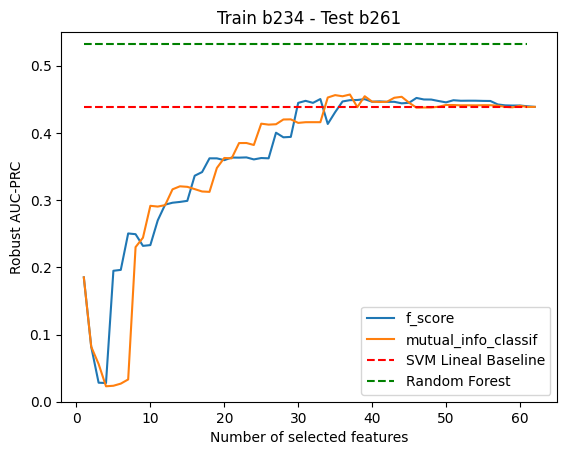
\includegraphics[width=0.25\textwidth]{Kap5/linear_ALL_METHODS_train=b234test=b261}  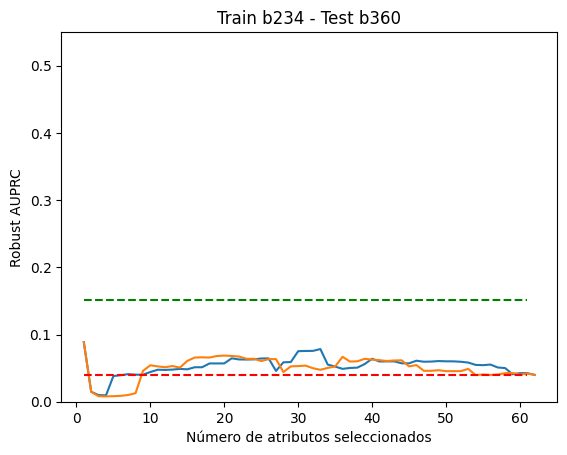
\includegraphics[width=0.25\textwidth]{Kap5/linear_ALL_METHODS_train=b234test=b360}
  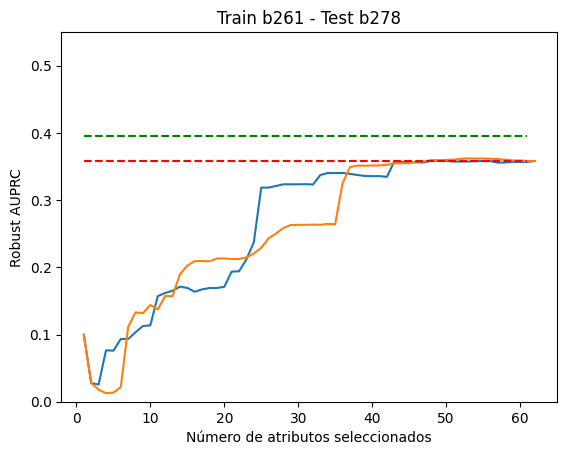
\includegraphics[width=0.25\textwidth]{Kap5/linear_ALL_METHODS_train=b261test=b278}  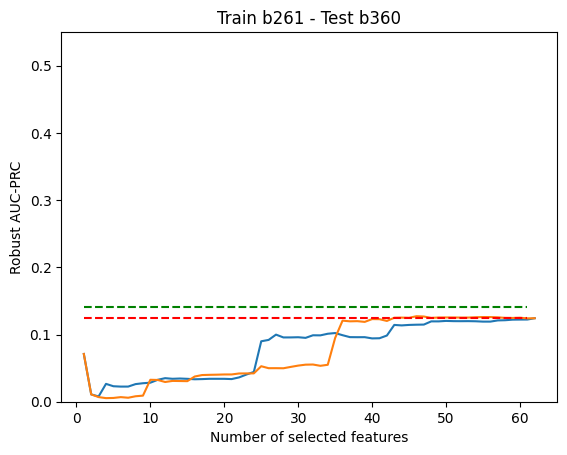
\includegraphics[width=0.25\textwidth]{Kap5/linear_ALL_METHODS_train=b261test=b360} \\

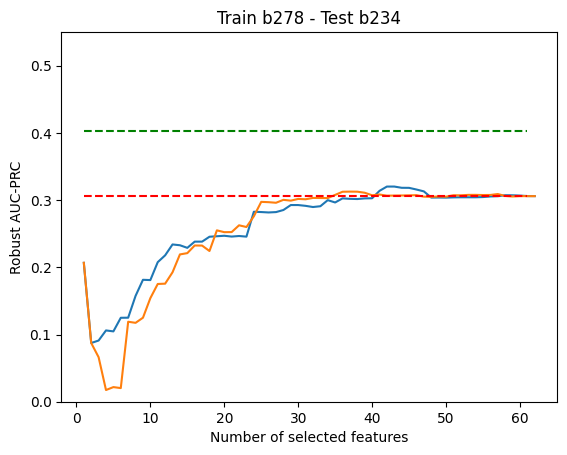
\includegraphics[width=0.25\textwidth]{Kap5/linear_ALL_METHODS_train=b278test=b234}  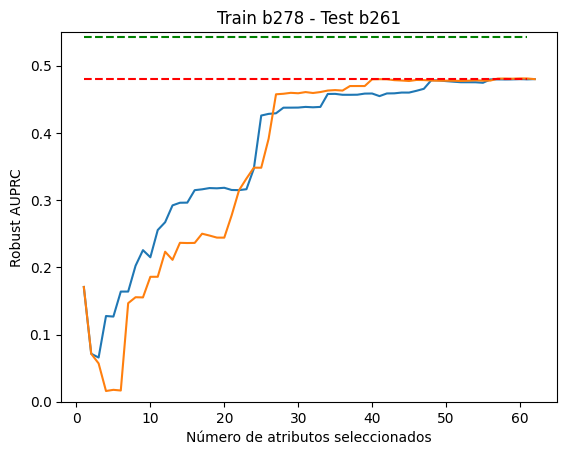
\includegraphics[width=0.25\textwidth]{Kap5/linear_ALL_METHODS_train=b278test=b261} 
 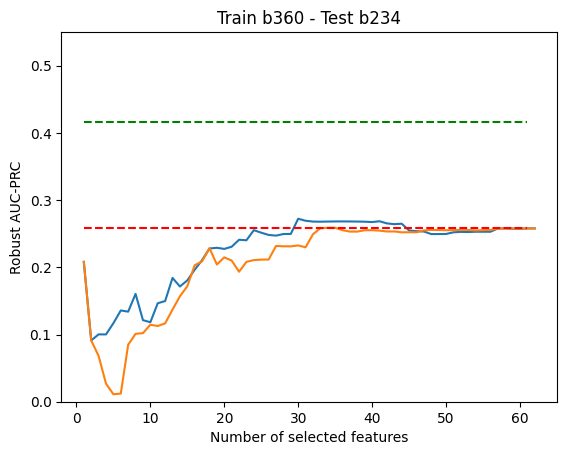
\includegraphics[width=0.25\textwidth]{Kap5/linear_ALL_METHODS_train=b360test=b234}  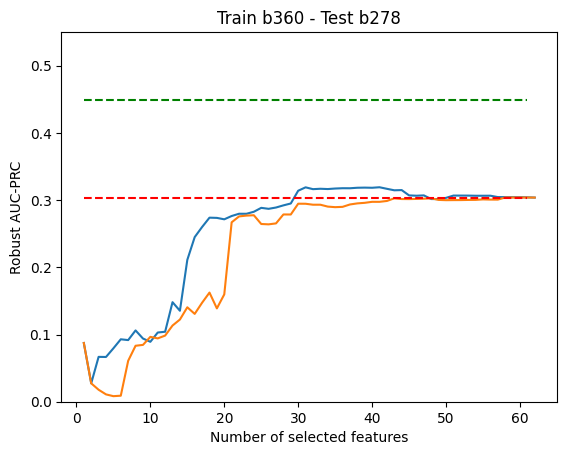
\includegraphics[width=0.25\textwidth]{Kap5/linear_ALL_METHODS_train=b360test=b278} 
\end{tabular}
\caption{Aplicación de filtros univariable en SVM-Lineal. Para cada par de tiles, se calcula el R-AUPRC de la curva de precision-recall en test obtenida entrenando con los $k$ atributos de mayor puntaje. La línea roja punteada es la performance de SVM sin usar selección de variables.}
\label{fig:svml_univariate}
\end{figure}

\begin{figure}[h!]
\begin{tabular}{cc}
  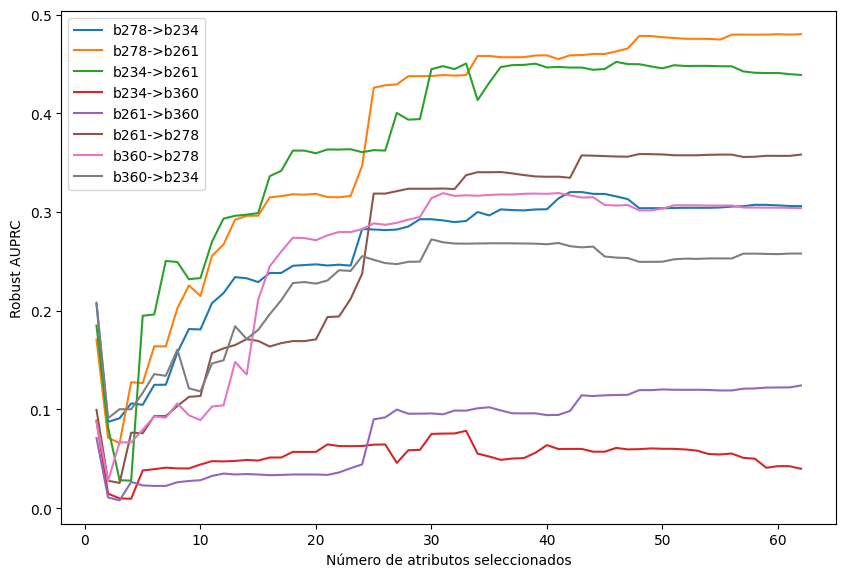
\includegraphics[width=0.49\textwidth]{Kap5/linear_f_classif_ALL_CURVES.png} &   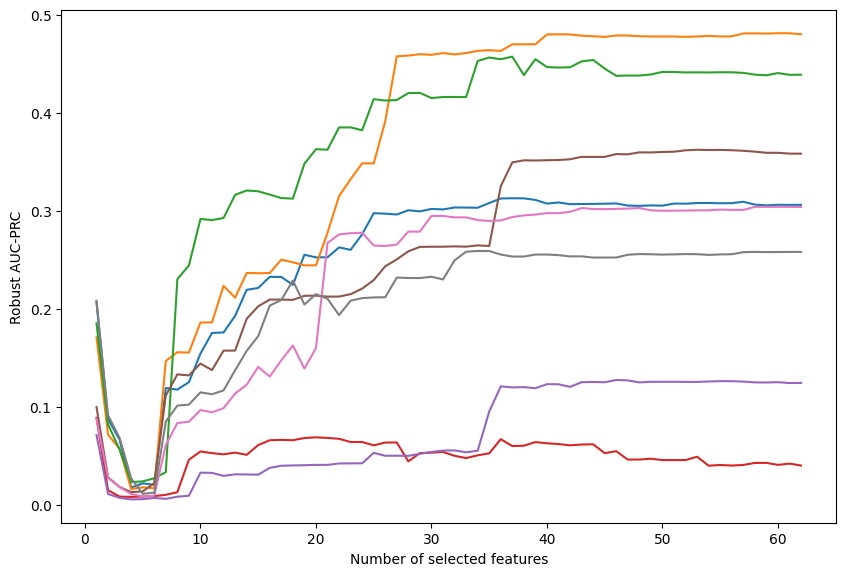
\includegraphics[width=0.49\textwidth]{Kap5/linear_mutual_info_classif_ALL_CURVES.png} \\
(a) Filtro: $f\_classif$ & (b) Filtro: $mutual\_info$
\end{tabular}
\caption{Aplicación de filtros univariable en SVM-Lineal en distintos pares de tiles. Nótese que las curvas tienden a saturarse al utilizar un número de atributos mucho menor al total de atributos (62), lo cuál indica que a partir de un cierto punto hay muy poco beneficio en agregar más atributos. }
\label{fig:svml_univariate_unified}
\end{figure}

Para elegir un valor óptimo de $k$ de forma analítica, se decidió calcular cuánto mejora (o empeora) el R-AUPRC para cada valor de $k$ respecto a no utilizar selección de variables. Dado que este análisis se realizó sobre 8 pares de tiles, en la figura \ref{fig:optimal_k_svml} se muestra el promedio de la diferencia entre el R-AUPRC utilizando k atributos y la base de referencia. Adicionalmente, en color naranja, se muestra la diferencia obtenida por aquel par de tiles que menos se beneficia para cada valor de $k$. \\

Esta gráfica nos permite entender qué valores de $k$ son más convenientes, o al menos no incurren en grandes pérdidas de R-AUPRC. Las conclusiones finales son:

\begin{itemize}
\item Ningún valor del hiperparámetro $k$ permite, en promedio, mejorar el R-AUPRC en todos los tiles. Por otro lado, es perfectamente posible igualar la performance de la base de referencia eliminando varios atributos.
\item Utilizando $f\_classif$, seleccionar 30 atributos no disminuye el R-AUPRC en promedio. Sin embargo, algunos tiles se ven altamente perjudicados, pues el mínimo toma valores negativos no despreciables. Seleccionar aproximadamente 50 atributos permitiría reducir esta variabilidad, obteniendo resultados más estables entre distintos pares de tiles.
\item Utilizando $mutual\_info$ podemos permitirnos seleccionar una cantidad menor de atributos ($k \geq 40$), garantizando que ningún par de tiles tendrá una pérdida significativa de R-AUPRC.
\end{itemize} 

\begin{figure}[h!]
\begin{tabular}{cc}
  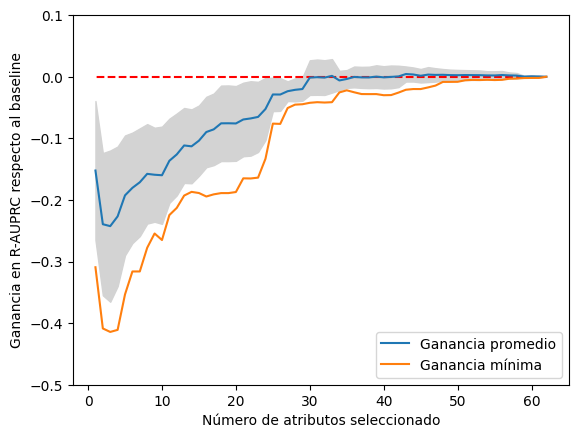
\includegraphics[width=0.49\textwidth]{Kap5/linearBEST_K_f_classif.png} &   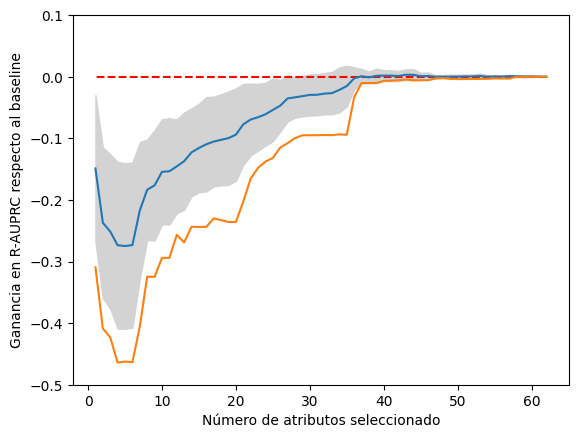
\includegraphics[width=0.49\textwidth]{Kap5/linearBEST_K_mutual_info_classif.png} \\
(a) Filtro: $f\_classif$ & (b) Filtro: $mutual\_info$
\end{tabular}
\caption{Estas gráficas permiten apreciar la diferencia en R-AUPRC respecto a la base de referencia, obtenida al realizar seleccionar $k$ atributos en SVM Lineal. Dado que esta diferencia se computó sobre 8 pares de tiles, para cada $k$ se muestra la media, la desviación estándar y el mínimo valor de entre todos los pares testeados. }
\label{fig:optimal_k_svml}
\end{figure}


\subsection{Experimentos en SVM-RBF}

En la figura \ref{fig:svmk_univariate} se encuentran los resultados de aplicar filtros univariable como paso previo a SVM-RBF. Las curvas muestran el impacto que tiene utilizar únicamente los $k$ atributos con mayor puntaje en el R-AUPRC. Podemos concluir que:

\begin{itemize}
\item Algunas curvas de SVM-RBF muestran una mejoría respecto a la base de referencia si se eliminan algunos atributos. 
\item Se puede reducir el tamaño del dataset aproximadamente a la mitad, seleccionando aproximadamente 30-35 atributos, mejorando o al menos no empeorando todas las curvas. 
\item Nótese que las curvas de SVM-Lineal comienzan a aplanarse a partir de $k=40$, en tanto que en las curvas de SVM-RBF (\ref{fig:svmk_univariate_unified}) tienden a aplanarse a partir de $k=30$. Esto sugiere que SVM-RBF genera superficies de decisión no lineales; y que hay relaciones no lineales involucradas en nuestros datos que SVM lineal no es capaz de capturar.
\end{itemize}

\begin{figure}[h!]
\begin{tabular}{cccc}
  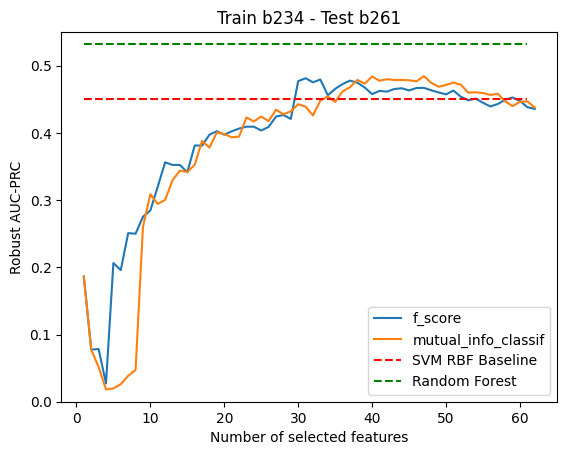
\includegraphics[width=0.25\textwidth]{Kap5/rbf_ALL_METHODS_train=b234test=b261}  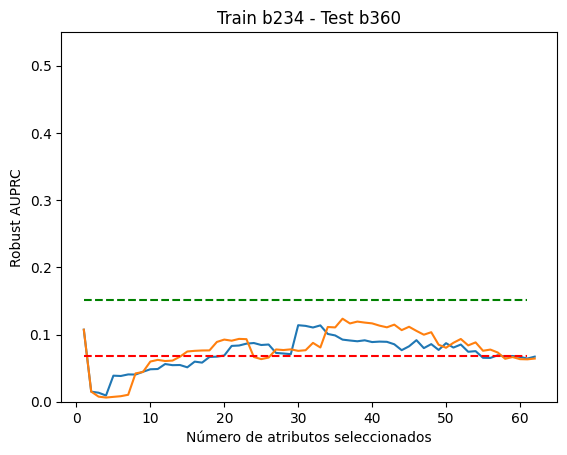
\includegraphics[width=0.25\textwidth]{Kap5/rbf_ALL_METHODS_train=b234test=b360}
  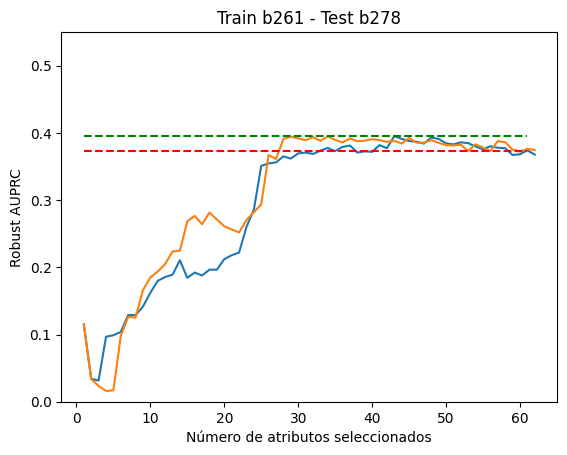
\includegraphics[width=0.25\textwidth]{Kap5/rbf_ALL_METHODS_train=b261test=b278}  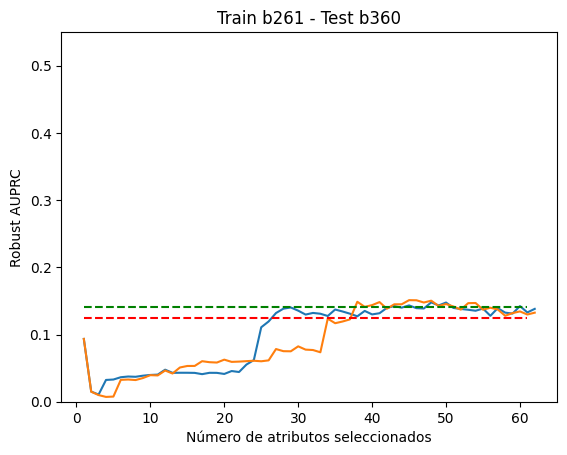
\includegraphics[width=0.25\textwidth]{Kap5/rbf_ALL_METHODS_train=b261test=b360} \\

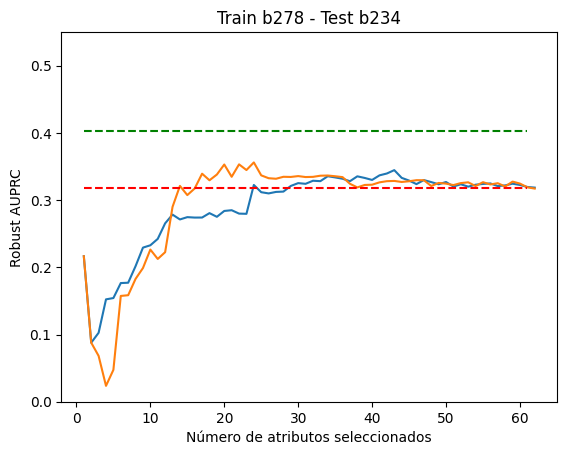
\includegraphics[width=0.25\textwidth]{Kap5/rbf_ALL_METHODS_train=b278test=b234}  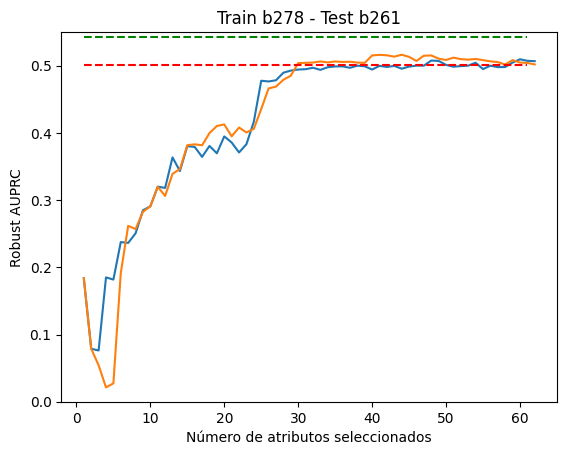
\includegraphics[width=0.25\textwidth]{Kap5/rbf_ALL_METHODS_train=b278test=b261} 
 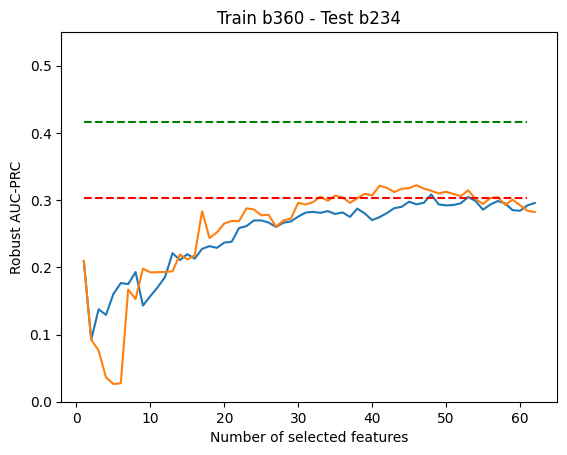
\includegraphics[width=0.25\textwidth]{Kap5/rbf_ALL_METHODS_train=b360test=b234}  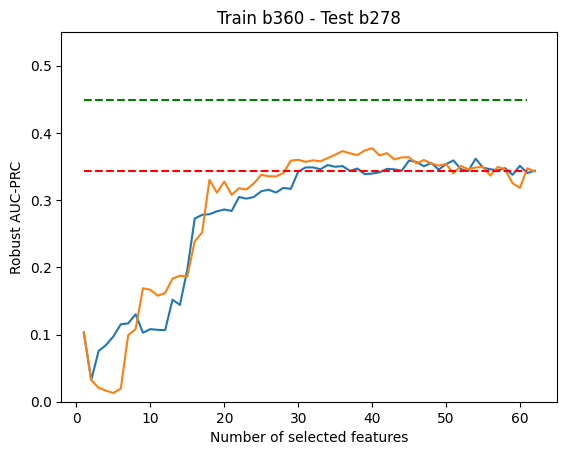
\includegraphics[width=0.25\textwidth]{Kap5/rbf_ALL_METHODS_train=b360test=b278} 
\end{tabular}
\caption{Aplicación de filtros univariable en SVM-RBF. Para cada par de tiles, se calcula el R-AUPRC de la curva de precision-recall en test obtenida entrenando con los $k$ atributos de mayor puntaje. La línea roja punteada es la performance de SVM sin usar selección de variables.}
\label{fig:svmk_univariate}
\end{figure}

\begin{figure}[h!]
\begin{tabular}{cc}
  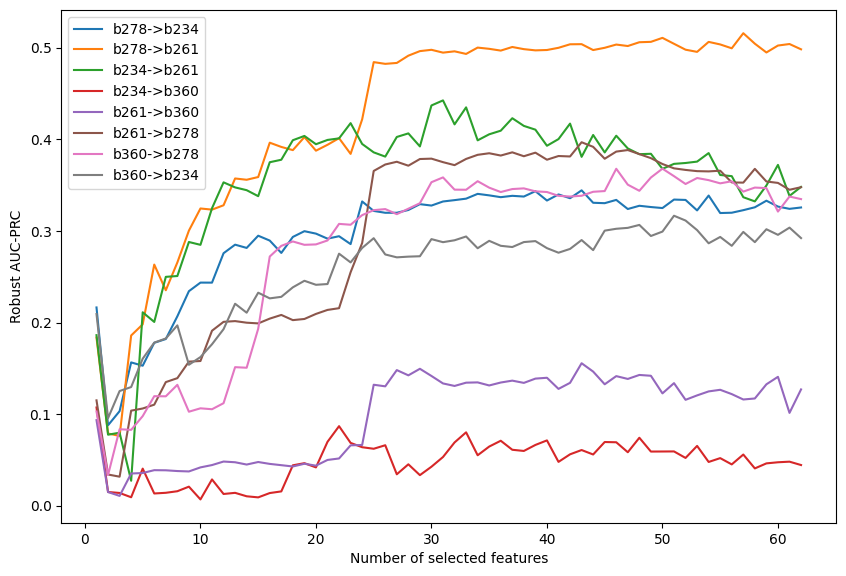
\includegraphics[width=0.49\textwidth]{Kap5/rbf_f_classif_ALL_CURVES.png} &   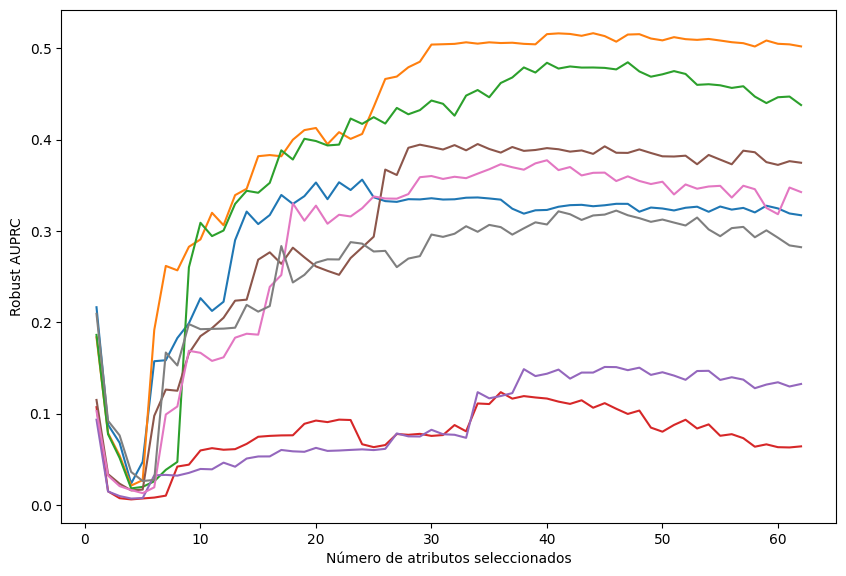
\includegraphics[width=0.49\textwidth]{Kap5/rbf_mutual_info_classif_ALL_CURVES.png} \\
(a) Filtro: $f\_classif$ & (b) Filtro: $mutual\_info$
\end{tabular}
\caption{Aplicación de filtros univariable en SVM-RBF en distintos pares de tiles.  Nótese que las curvas tienden a saturarse al utilizar un número de atributos mucho menor al total de atributos (62), lo cuál indica que a partir de un cierto punto hay muy poco beneficio en agregar más atributos.}
\label{fig:svmk_univariate_unified}
\end{figure}

Nuevamente, resulta complicado determinar el número óptimo de atributos a seleccionar a simple vista. Se procedió a resumir la información de las 8 curvas en la figura \ref{fig:optimal_k_svmk}, que analiza la ganancia promedio en R-AUPRC para cada $k$. Las conclusiones finales son:

\begin{itemize}
\item Seleccionar $35 \leq k \leq 55$ atributos de acuerdo al ranking de $mutual\_info$ permite mejorar el R-AUPRC respecto a la base de referencia en \textit{todos} los pares testeados. En particular, $k=45$ maximiza la mínima diferencia y el promedio.
\item Seleccionar variables de acuerdo al criterio $f\_classif$ es menos beneficioso, pues existen pocos valores de $k$ para los cuales el R-AUPRC no empeora en ningún par de tiles testeado; y la mejora es un poco más modesta que la observada utilizando $mutual\_info$. Esto puede deberse a que $f\_classif$ es incapaz de detectar correlaciones no lineales, y puede estar causando el descarte prematuro de variables que resultan útiles a SVM-RBF para detectar RRLs.
\end{itemize}

\begin{figure}[h!]
\begin{tabular}{cc}
  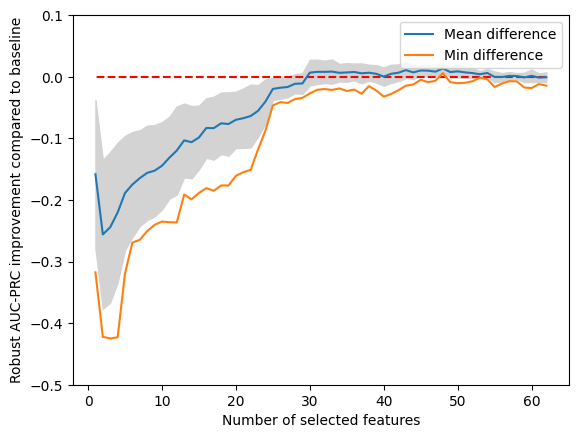
\includegraphics[width=0.49\textwidth]{Kap5/rbfBEST_K_f_classif.png} &   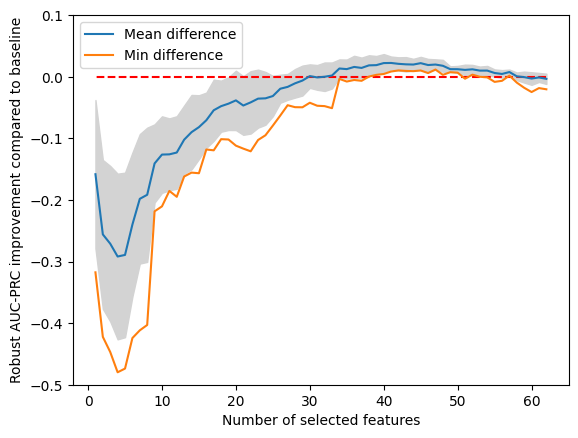
\includegraphics[width=0.49\textwidth]{Kap5/rbfBEST_K_mutual_info_classif.png} \\
(a) Filtro: $f\_classif$ & (b) Filtro: $mutual\_info$
\end{tabular}
\caption{Estas gráficas permiten apreciar la diferencia en R-AUPRC respecto a la base de referencia, obtenida al realizar seleccionar $k$ atributos en SVM-RBF. Dado que esta diferencia se computó sobre 8 pares de tiles, para cada $k$ se muestra la media, la desviación estándar y el mínimo valor de entre todos los pares testeados. }
\label{fig:optimal_k_svmk}
\end{figure}

\section{Extracción de variables}

\subsection{Introducción a extracción de variables}

Consideremos un cierto fenómeno gobernado por $L$ variables independientes. En la práctica, este fenómeno probablemente aparentará tener muchos más grados de libertad, debido a la influencia de factores como ruido, imperfección en el sistema de mediciones, adición de atributos irrelevantes, etcétera. Se define la \textbf{dimensión intrínseca} de un fenómeno como el \textit{número de variables independientes que explica satisfactoriamente ese 
fenómeno}\cite{carreira}. \\

Dado un dataset $X$ con $d$ atributos numéricos, extracción de variables consiste en hallar un mapeo $\mathds{R}^d \mapsto \mathds{R}^p$ con $p \leq d$; donde idealmente $p$ será la dimensionalidad intrínseca de X. Este mapeo es utilizado para encontrar una representación más compacta de $X$ sin perder información \cite{fextraction}. Al igual que en selección de variables, se espera obtener un beneficio en términos de desempeño y eficiencia. Adicionalmente, los datos pueden ser más fáciles de visualizar o separar en el nuevo espacio. \\

Los métodos de extracción de variables pueden clasificarse en dos tipos \cite{fextraction}: 
\begin{itemize}
\item \textbf{Supervisados}: Tienen en cuenta las etiquetas (clases) de cada instancia a proyectar.
\item \textbf{No supervisados}: No tienen en cuenta la separación entre clases, y se concentran principalmente en la variación y distribución de los datos.
\end{itemize}

\subsection{Principal Component Analysis}

\label{PCA}

En esta sección se describirá un método de extracción de variables no supervizado muy popular: Principal Component Analysis (PCA) \cite{han2012mining}. \\

Supongamos que se desea reducir la cantidad de variables de un dataset $X$ descripto por $p$ atributos. Se definen las \textbf{componentes principales} de $X$ como la secuencia de $p$ vectores unitarios, donde el $i$-ésimo vector es la dirección que mejor ajusta los datos en tanto que es ortogonal a los primeros $i-1$ vectores. En este contexto, la dirección o línea que mejor ajusta los datos es definida como aquella que minimiza la distancia cuadrada promedio de todos los puntos a la línea. \\

Estas direcciones constituyen una base ortonormal en la cual las distintas dimensiones individuales están linealmente decorrelacionadas.  Equivalentemente, la $i$-ésima componente principal puede ser definida como la dirección ortogonal a las primeras $i-1$ componentes principales que maximiza la varianza de los datos proyectados. En la figura \ref{fig:pca} se puede ver un ejemplo ilustrativo.  \\

\begin{figure}[h!]
\centering
  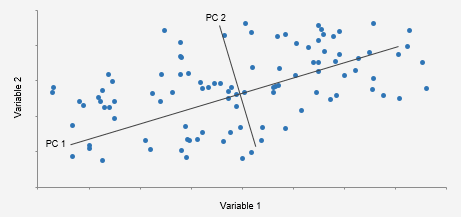
\includegraphics[width=0.49\textwidth]{Kap5/pca.png}
\caption{En esta imagen se ilustran las dos componentes principales de un conjunto de datos bidimensional. La primer componente principal es aquella que maximiza la varianza de los datos proyectados, o, equivalentemente, la dirección que define la recta que mejor ajusta los datos. Nótese que las etiquetas de los datos no son utilizadas. Créditos: \url{statistixl.com}}
\label{fig:pca}
\end{figure}

\textbf{PCA} es el proceso de computar las componentes principales y usarlas para realizar un cambio de base en los datos, usualmente utilizando sólo las primeras $k<p$ componentes principales e ignorando las restantes. \\

En la figura \ref{fig:pca_l} podemos ver el impacto de aplicar PCA como paso previo a SVM Lineal, en tanto que en la \ref{fig:pca_k} se pueden apreciar los resultados del experimento equivalente en SVM RBF. Es importante remarcar que se calcula la transformación únicamente sobre los datos de entrenamiento, y esta misma transformación es aplicada a los datos de test.\\

Podemos ver que el uso de PCA tiene un efecto muy dispar en distintos pares de tiles testeados. Para ciertas combinaciones, utilizar PCA conduce a mejoras muy significativas, llegando a superar incluso la performance obtenida por Random Forests. Sin embargo, para otros pares de tiles el R-AUPRC disminuye drásticamente, lo cuál nos lleva a descartar este preprocesamiento para experimentos futuros.

\begin{figure}[h!]
\begin{tabular}{cccc}
  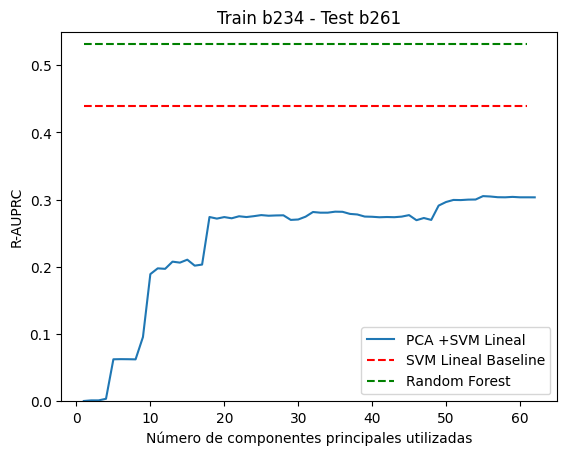
\includegraphics[width=0.25\textwidth]{Kap5/linear_INDIVIDUAL_CURVES_train=b234test=b261.png}  
  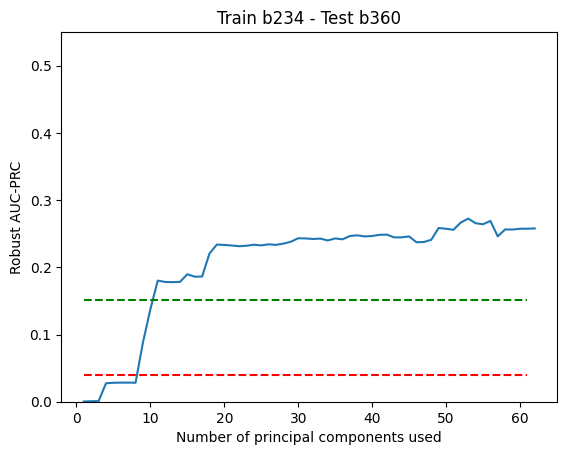
\includegraphics[width=0.25\textwidth]{Kap5/linear_INDIVIDUAL_CURVES_train=b234test=b360.png}
  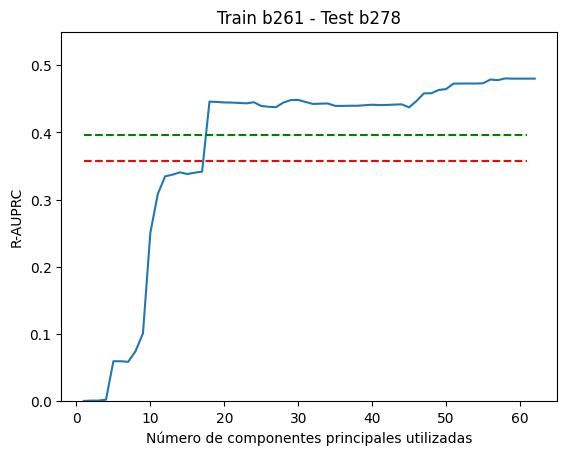
\includegraphics[width=0.25\textwidth]{Kap5/linear_INDIVIDUAL_CURVES_train=b261test=b278.png}  
  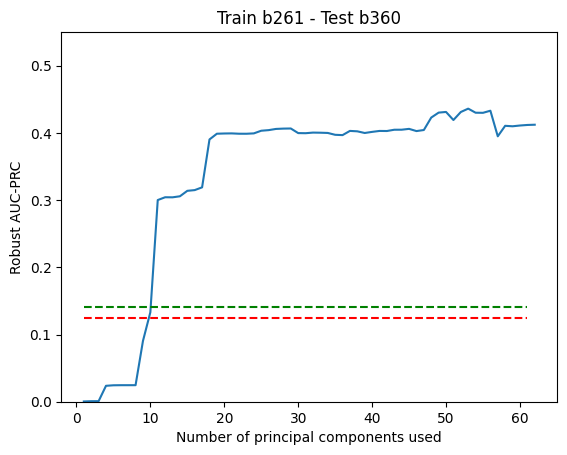
\includegraphics[width=0.25\textwidth]{Kap5/linear_INDIVIDUAL_CURVES_train=b261test=b360.png} \\

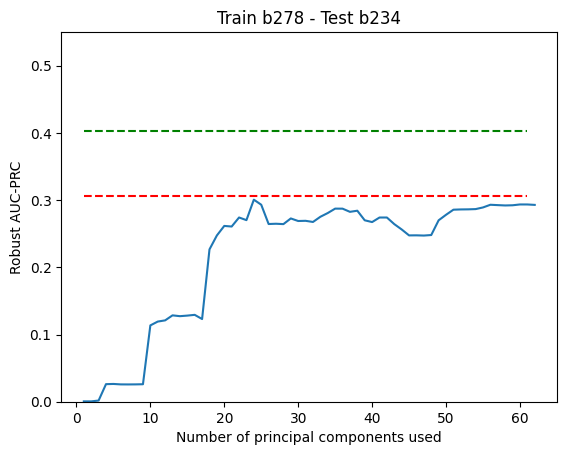
\includegraphics[width=0.25\textwidth]{Kap5/linear_INDIVIDUAL_CURVES_train=b278test=b234.png}  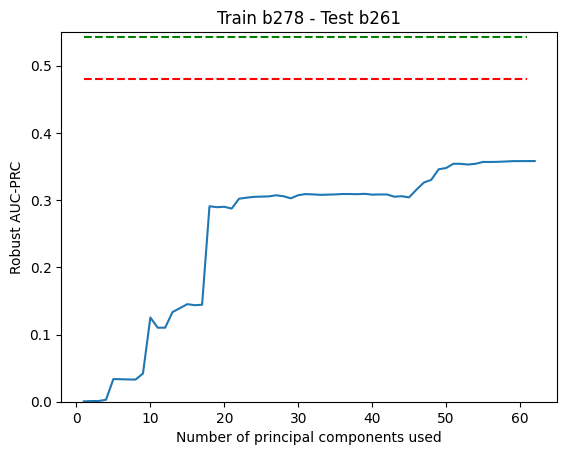
\includegraphics[width=0.25\textwidth]{Kap5/linear_INDIVIDUAL_CURVES_train=b278test=b261.png} 
 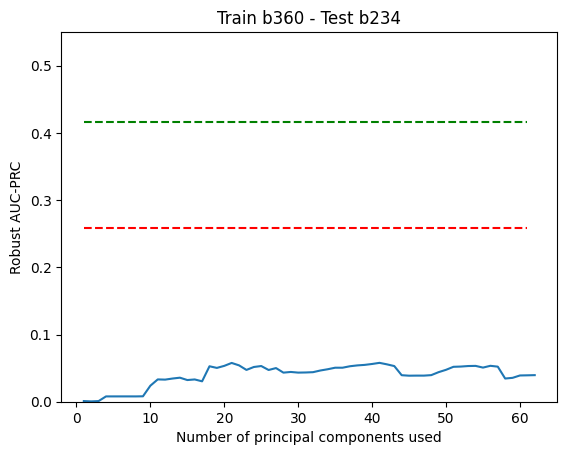
\includegraphics[width=0.25\textwidth]{Kap5/linear_INDIVIDUAL_CURVES_train=b360test=b234.png}  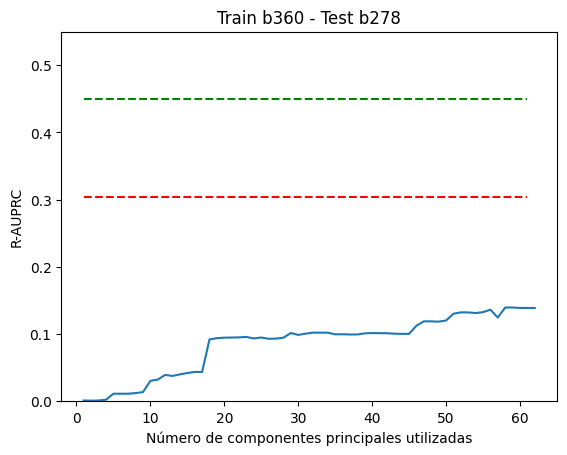
\includegraphics[width=0.25\textwidth]{Kap5/linear_INDIVIDUAL_CURVES_train=b360test=b278.png} 
\end{tabular}
\caption{Aplicación de PCA a SVM Lineal. Para cada par de tiles, se muestra el R-AUPRC obtenido al entrenar y testear usando las primeras $k$ componentes principales. La línea punteada roja representa la base de referencia de SVM, obtenido sin utilizar extracción de variables. La línea verde punteada representa la performance de RF.}
\label{fig:pca_l}
\end{figure}

\begin{figure}[h!]
\begin{tabular}{cccc}
  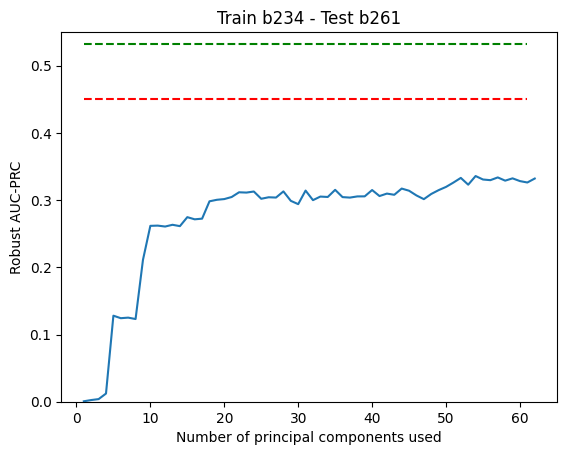
\includegraphics[width=0.25\textwidth]{Kap5/rbf_INDIVIDUAL_CURVES_train=b234test=b261.png}  
  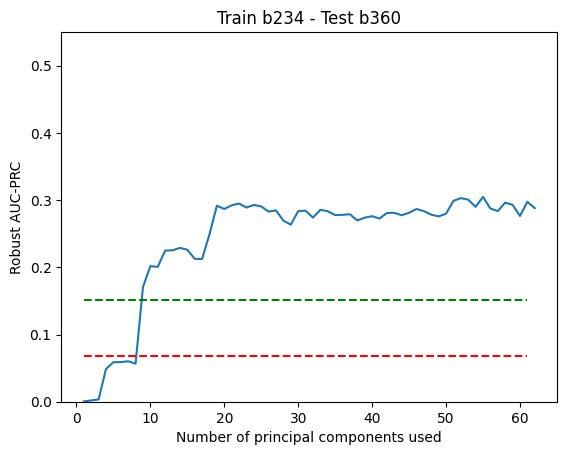
\includegraphics[width=0.25\textwidth]{Kap5/rbf_INDIVIDUAL_CURVES_train=b234test=b360.png}
  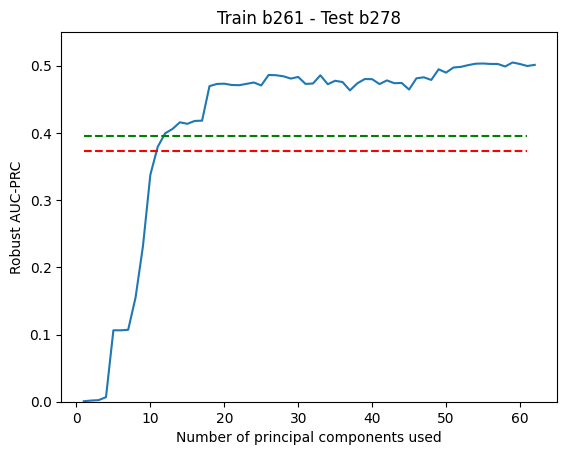
\includegraphics[width=0.25\textwidth]{Kap5/rbf_INDIVIDUAL_CURVES_train=b261test=b278.png}  
  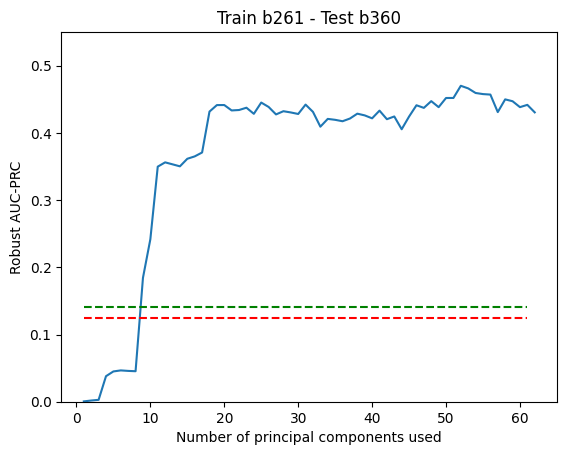
\includegraphics[width=0.25\textwidth]{Kap5/rbf_INDIVIDUAL_CURVES_train=b261test=b360.png} \\

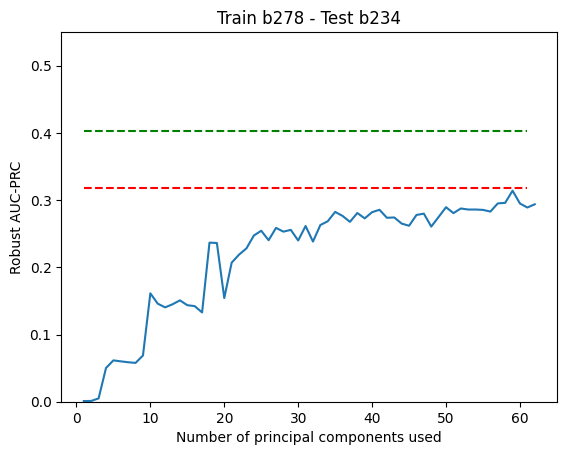
\includegraphics[width=0.25\textwidth]{Kap5/rbf_INDIVIDUAL_CURVES_train=b278test=b234.png}  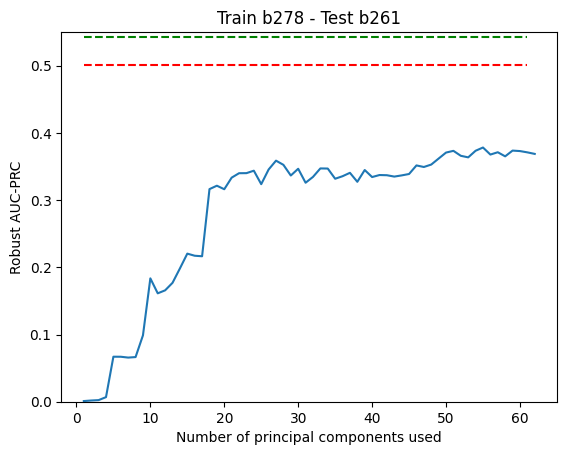
\includegraphics[width=0.25\textwidth]{Kap5/rbf_INDIVIDUAL_CURVES_train=b278test=b261.png} 
 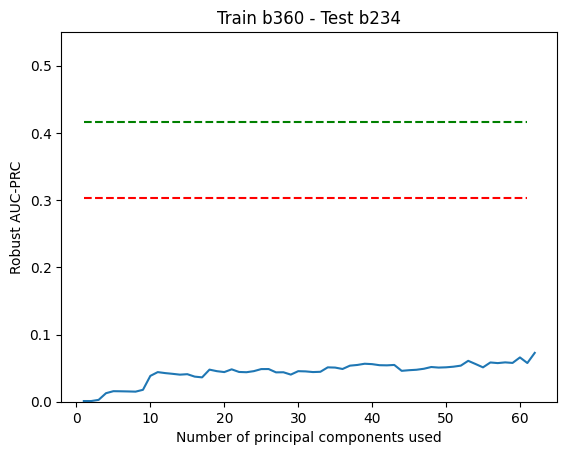
\includegraphics[width=0.25\textwidth]{Kap5/rbf_INDIVIDUAL_CURVES_train=b360test=b234.png}  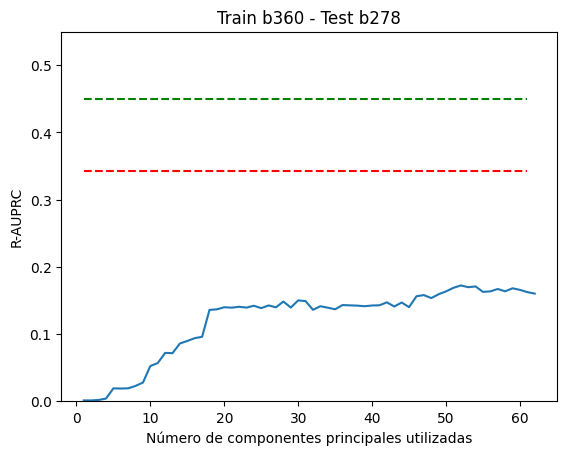
\includegraphics[width=0.25\textwidth]{Kap5/rbf_INDIVIDUAL_CURVES_train=b360test=b278.png} 
\end{tabular}
\caption{Aplicación de PCA a SVM RBF. Para cada par de tiles, se muestra el R-AUPRC obtenido al entrenar y testear usando las primeras $k$ componentes principales. La línea punteada roja representa el R-AUPRC de SVM-RBF obtenido sin utilizar extracción de variables. La línea verde punteada representa la performance de RF.}
\label{fig:pca_k}
\end{figure}

\subsection{Clustering de variables}

En esta sección se aplicó un último método de extracción de variables no supervisado, llamado \textbf{clustering de variables}. En primer lugar, se introducirán brevemente algunos conceptos de aprendizaje automatizado no supervisado para poder describir esta técnica. \\

Dado un dataset no etiquetado $X$ con $n$ elementos, la tarea de \textbf{clustering} \cite{Jain88} consiste en dividir los $n$ objetos en grupos, de tal forma que todos los objetos en un mismo grupo (\textit{cluster}) son más similares (en algún sentido) a aquellos que están en otros grupos (\textit{clusters}). \\

Aquellas técnicas que construyen un anidado o jerarquía de clusters pertenecen al grupo de técnicas de \textbf{clustering jerárquico} \cite{Jain88} \cite{clustering}. Esto se ilustra en la figura \ref{fig:jerarquico}. \\

\begin{figure}[h!]
\begin{center}
 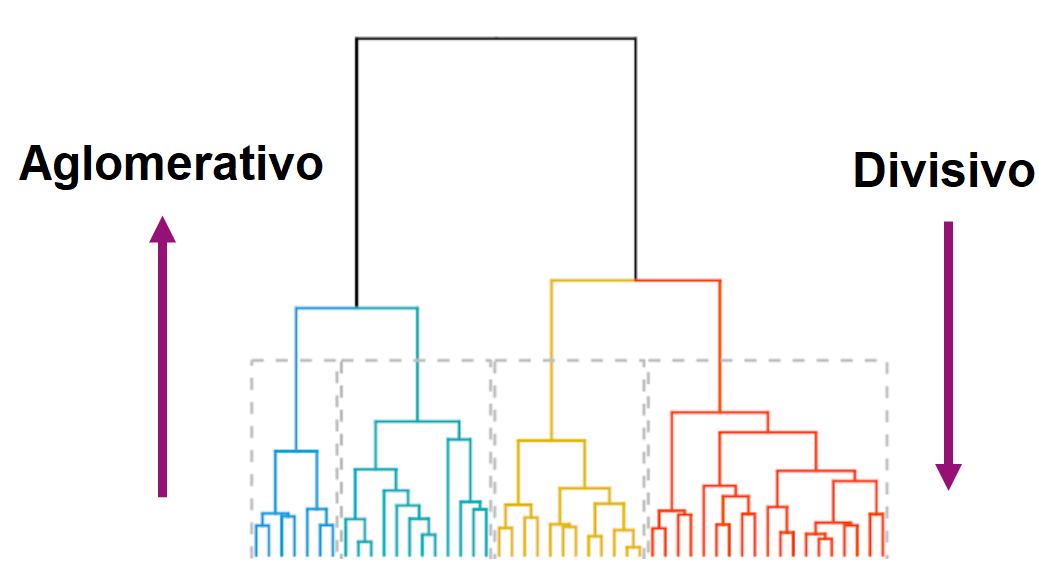
\includegraphics[width=0.6\textwidth]{Kap5/jerarquico.png}
\end{center}

\caption{Ejemplo de clustering jerárquico. Los elementos de un cierto dataset se agrupan en clusters que recursivamente pueden pertenecer a otros clusters. Créditos: Towards Data Science.}
\label{fig:jerarquico}
\end{figure}

Los algoritmos de clustering jerárquico generalmente se dividen en dos grandes grupos \cite{clustering} \cite{iretrieval} :

\begin{itemize}
\item \textbf{Aglomerativos} (Bottom-up): Cada elemento del dataset comienza en su propio cluster, y pares de clusters son combinados recursivamente.
\item \textbf{Divisivos} (Top-down):  Todos los elementos del dataset comienzan en un mismo cluster, y divisiones son realizadas recursivamente.
\end{itemize}

En esta sección nos concentraremos en algoritmos de clustering jerárquico aglomerativos, que iterativamente combinan el par de clusters que minimiza una cierta métrica de disimilitud \cite{clustering}. En este experimento se utilizaron las siguientes métricas de disimilitud:

\begin{itemize}
\item \textbf{Single linkage}: La distancia mínima entre pares de puntos, uno en cada cluster \cite{iretrieval}. Esta métrica busca conectividad, no grupos compactos.   

\item \textbf{Complete linkage}: La distancia máxima entre pares de puntos, uno en cada cluster \cite{iretrieval}. Intuitivamente, esta métrica busca agrupar conjuntos \textit{completamente vecinos}, formando clusters compactos. 

\item \textbf{Average linkage}: Promedio de las distancias entre todas las observaciones de pares de clusters \cite{iretrieval}. Esta métrica busca grupos conectados y compactos.

\item \textbf{Ward}: Minimiza la suma de las diferencias cuadradas dentro de todos los clusters \cite{ward}. Es un enfoque que busca minimizar la varianza.
\end{itemize}

En la figura \ref{fig:linkages} se pueden observar los clusters generados por las cuatro métricas explicadas en tres datasets ilustrativos. \\

\begin{figure}[h!]
 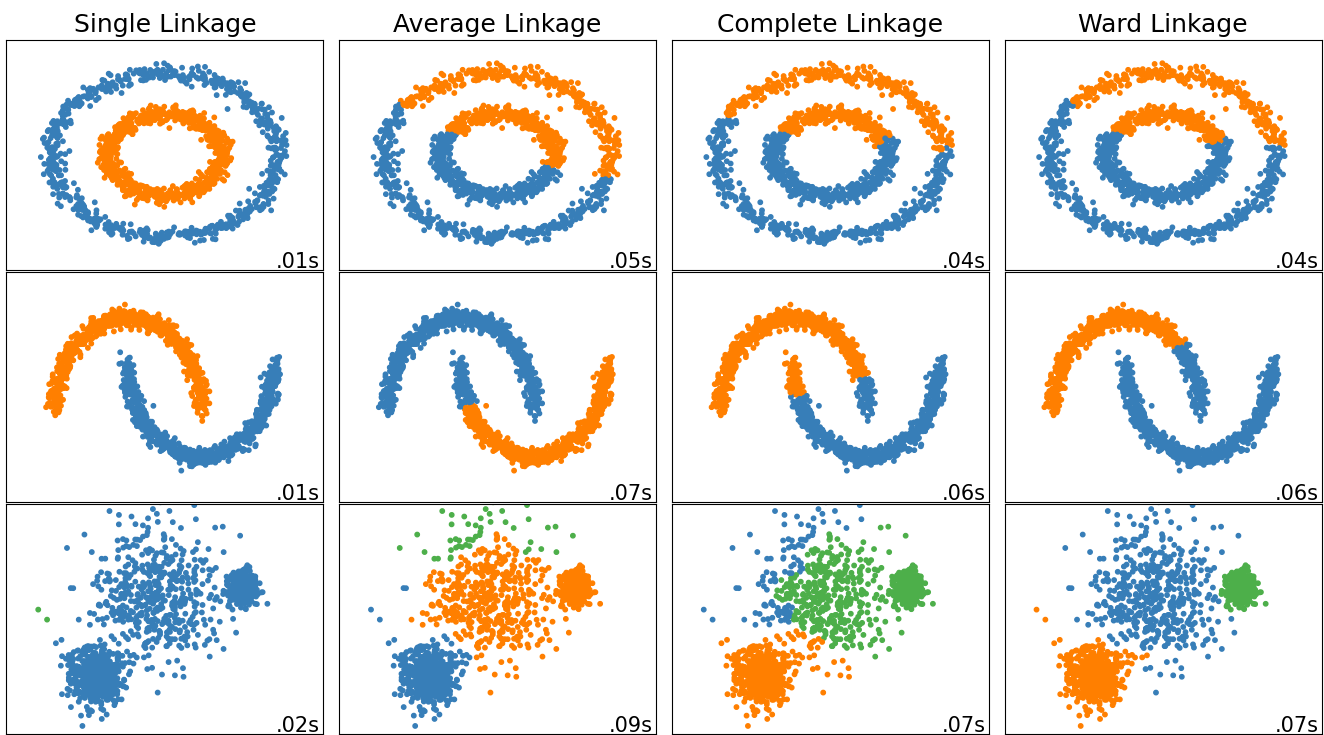
\includegraphics[width=\textwidth]{Kap5/jerarquico_tecnicas.png}
\caption{Efecto de distintas métricas de similitud en clustering jerárquico. Imagen tomada de la documentación oficial de Sklearn.}
\label{fig:linkages}
\end{figure}

En esta sección se aplicó clustering para combinar atributos, en lugar de elementos de un dataset. En clustering aglomerativo estándar, el algoritmo recibe un dataset con $n$ elementos descriptos por $m$ atributos representado por una matriz $M \in \mathbf{R}^{n \times m}$. En \textbf{clustering de variables} (feature agglomeration, en inglés) \cite{fs3}, el algoritmo de clustering aglomerativo simplemente recibe como argumento la transpuesta del dataset, $M^T$, e intentará combinar atributos que se comportan de forma similar, reemplazándolos por el centroide del cluster\footnote{Usualmente se utiliza el promedio, aunque se podría una función arbitraria (llamada \textit{pooling function}) para definir cómo unificar clusters }. \\

Los resultados de estos experimentos pueden verse en las figuras \ref{fig:agg_l} y \ref{fig:agg_k} para SVM lineal y SVM RBF respectivamente. Las curvas generadas son notablemente similares a las obtenidas utilizando PCA. \\

La métrica de disimilaridad utilizada para hallar clústers no tiene un gran impacto en las curvas generadas. Al igual que en PCA, utilizar clustering de variables produce aumentos muy interesantes de R-AUPRC en ciertos pares de tiles y desmejorías notables en otros; es por esto que se decidió no utilizar esta técnica en secciones posteriores.

\begin{figure}[h!]
\begin{tabular}{cccc}
  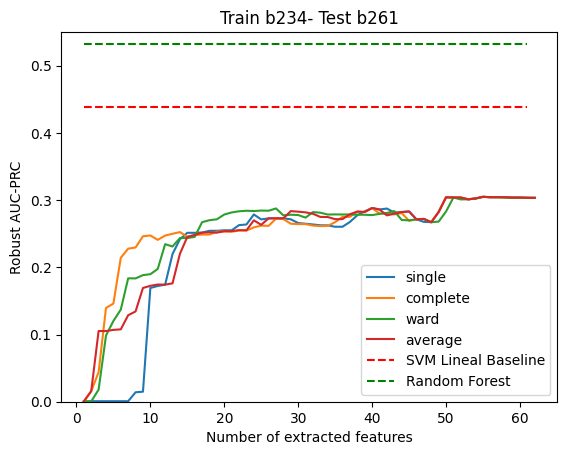
\includegraphics[width=0.25\textwidth]{Kap5/linear_ALL_LINKAGES_train=b234test=b261.png}  
  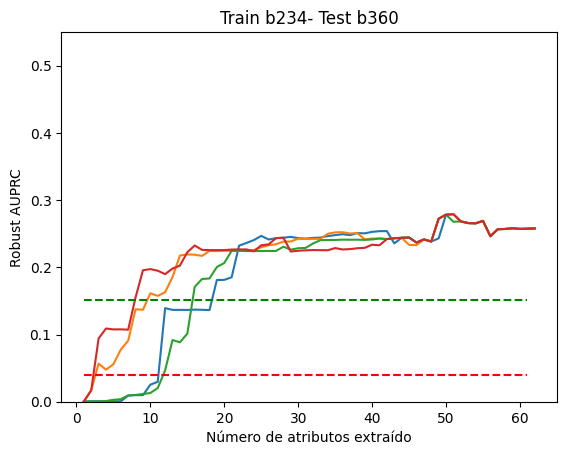
\includegraphics[width=0.25\textwidth]{Kap5/linear_ALL_LINKAGES_train=b234test=b360.png}
  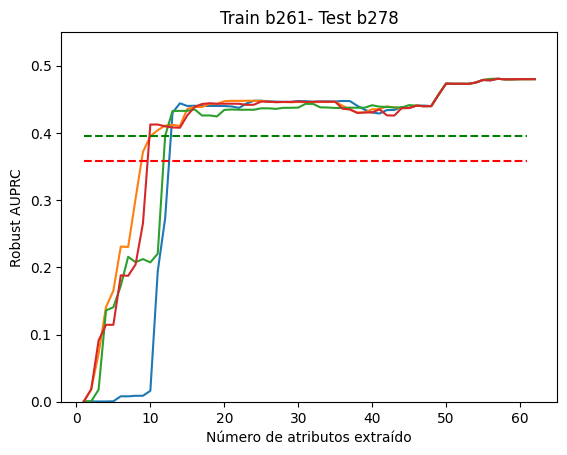
\includegraphics[width=0.25\textwidth]{Kap5/linear_ALL_LINKAGES_train=b261test=b278.png}  
  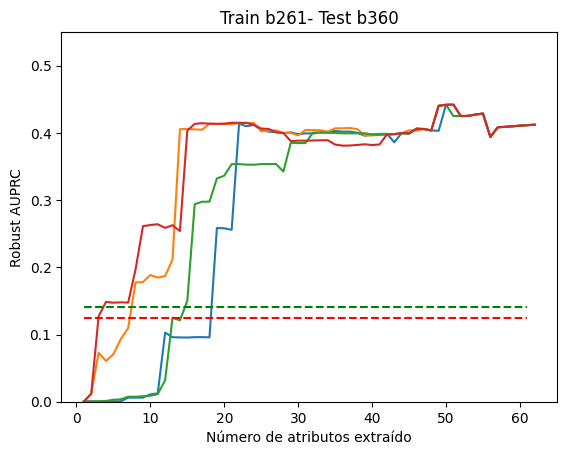
\includegraphics[width=0.25\textwidth]{Kap5/linear_ALL_LINKAGES_train=b261test=b360.png} \\

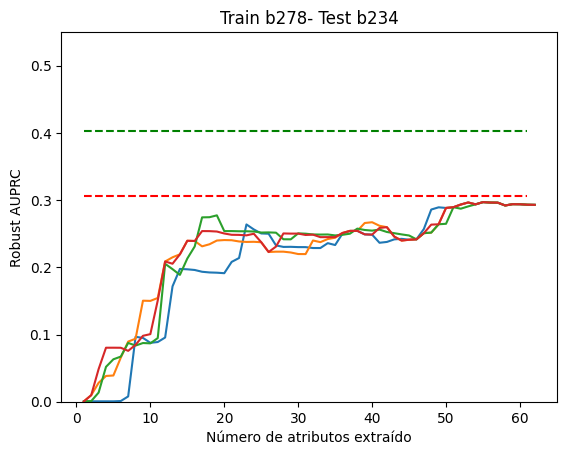
\includegraphics[width=0.25\textwidth]{Kap5/linear_ALL_LINKAGES_train=b278test=b234.png}  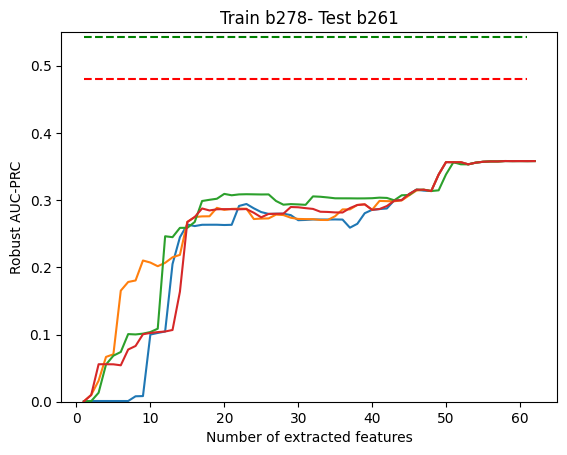
\includegraphics[width=0.25\textwidth]{Kap5/linear_ALL_LINKAGES_train=b278test=b261.png} 
 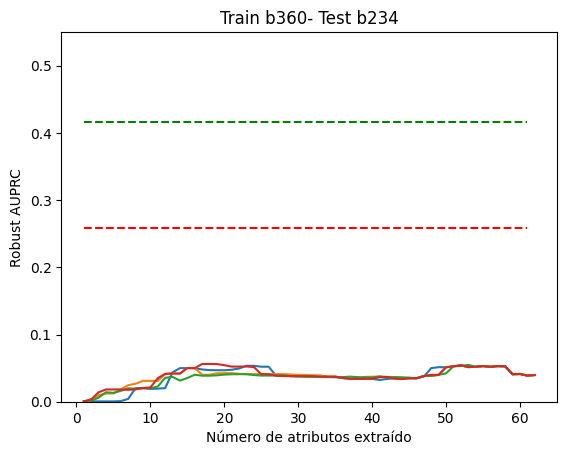
\includegraphics[width=0.25\textwidth]{Kap5/linear_ALL_LINKAGES_train=b360test=b234.png}  \includegraphics[width=0.25\textwidth]{Kap5/linear_ALL_LINKAGES_train=b360test=b278.png} 
\end{tabular}
\caption{Aplicación de clustering de variables a SVM Lineal}
\label{fig:agg_l}
\end{figure}

\begin{figure}[h!]
\begin{tabular}{cccc}
  \includegraphics[width=0.25\textwidth]{Kap5/rbf_ALL_LINKAGES_train=b234test=b261.png}  
  \includegraphics[width=0.25\textwidth]{Kap5/rbf_ALL_LINKAGES_train=b234test=b360.png}
  \includegraphics[width=0.25\textwidth]{Kap5/rbf_ALL_LINKAGES_train=b261test=b278.png}  
  \includegraphics[width=0.25\textwidth]{Kap5/rbf_ALL_LINKAGES_train=b261test=b360.png} \\

\includegraphics[width=0.25\textwidth]{Kap5/rbf_ALL_LINKAGES_train=b278test=b234.png}  \includegraphics[width=0.25\textwidth]{Kap5/rbf_ALL_LINKAGES_train=b278test=b261.png} 
 \includegraphics[width=0.25\textwidth]{Kap5/rbf_ALL_LINKAGES_train=b360test=b234.png}  \includegraphics[width=0.25\textwidth]{Kap5/rbf_ALL_LINKAGES_train=b360test=b278.png} 
\end{tabular}
\caption{Aplicación de clustering de variables a SVM RBF}
\label{fig:agg_k}
\end{figure}

\section{Conclusiones}
\label{mejores_fs}
En este capítulo se han explorado distintas técnicas para reducir la dimensionalidad de los datos. Ninguna de las técnicas estudiadas tuvo un impacto pronunciado en las curvas de precision-recall, por lo que la aplicación de estos métodos tiene sentido principalmente para reducir la complejidad temporal y espacial de nuestros clasificadores. \\

Dado que las técnicas de extracción de variables probaron generar resultados bastante inestables, se decidió preferir el uso de selección de variables (filtros univariable) en el resto de este trabajo. En base a los valores graficados en las figuras \ref{fig:optimal_k_svml} y \ref{fig:optimal_k_svmk}, se decidió optar por aquellos hiperparámetros que maximizan la ganancia promedio en R-AUPRC, sujeto a no empeorar significativamente la performance en ningún par de tiles.

\begin{itemize}
\item Seleccionar los 48 atributos más importantes de acuerdo a $mutual\_info$ en SVM-Lineal.
\item Seleccionar los 45 atributos más importantes de acuerdo a $mutual\_info$ en SVM-RBF.
\end{itemize}

En las tablas \ref{tab:fs_comparison_l} y \ref{tab:fs_comparison_r} podemos ver el impacto final de esta elección en R-AUPRC en SVM lineal y RBF respectivamente, en comparación a los clasificadores óptimos del capítulo anterior. La mejora en R-AUPRC es nula en SVM Lineal y modesta en SVM-RBF, y viene acompañada de una reducción en complejidad temporal y espacial. Esto último es especialmente notable en SVM-RBF, donde los tiempos de entrenamiento se redujeron significativamente.
 
\begin{table}[h!]
\centering
\begin{tabular}{|c|c|c|c|c|c|}
\hline
\textbf{Train tile} & \textbf{Test tile} & \textbf{RF} & \textbf{SVM-L sin FS} & \textbf{SVM-L con FS} & \textbf{Gain} \\ \hline
b278                & b234               & 0.40        & 0.31                  & 0.31                  & 0.00          \\ \hline
b278                & b261               & 0.54        & 0.48                  & 0.48                  & -0.00         \\ \hline
b278                & b360               & 0.21        & 0.14                  & 0.13                  & -0.00         \\ \hline
b234                & b278               & 0.40        & 0.29                  & 0.30                  & 0.01          \\ \hline
b234                & b261               & 0.53        & 0.44                  & 0.44                  & 0.00          \\ \hline
b234                & b360               & 0.15        & 0.04                  & 0.04                  & 0.00          \\ \hline
b261                & b278               & 0.40        & 0.36                  & 0.36                  & -0.00         \\ \hline
b261                & b234               & 0.39        & 0.30                  & 0.30                  & -0.00         \\ \hline
b261                & b360               & 0.14        & 0.12                  & 0.12                  & 0.00          \\ \hline
b360                & b278               & 0.45        & 0.30                  & 0.30                  & -0.00         \\ \hline
b360                & b234               & 0.42        & 0.26                  & 0.25                  & -0.00         \\ \hline
b360                & b261               & 0.54        & 0.41                  & 0.41                  & -0.01         \\ \hline
\multicolumn{2}{|c|}{avg}                & 0.38        & 0.29                  & 0.29                  & 0             \\ \hline
\end{tabular}
\caption{En esta tabla podemos ver el incremento nulo en R-AUPRC que se obtiene al utilizar selección de variables en SVM-Lineal. }
\label{tab:fs_comparison_l} 
\end{table}

\begin{table}[]
\centering
\begin{tabular}{|c|c|c|c|c|c|}
\hline
\textbf{Train tile} & \textbf{Test tile} & \textbf{RF} & \textbf{SVM-RBF sin FS} & \textbf{SVM-RBF con FS} & \textbf{Gain} \\ \hline
b278                & b234               & 0.40        & 0.32                    & 0.33                    & 0.01          \\ \hline
b278                & b261               & 0.54        & 0.50                    & 0.52                    & 0.02          \\ \hline
b278                & b360               & 0.21        & 0.16                    & 0.18                    & 0.02          \\ \hline
b234                & b278               & 0.40        & 0.30                    & 0.34                    & 0.04          \\ \hline
b234                & b261               & 0.53        & 0.45                    & 0.47                    & 0.02          \\ \hline
b234                & b360               & 0.15        & 0.07                    & 0.09                    & 0.02          \\ \hline
b261                & b278               & 0.40        & 0.37                    & 0.39                    & 0.02          \\ \hline
b261                & b234               & 0.39        & 0.33                    & 0.33                    & 0.00          \\ \hline
b261                & b360               & 0.14        & 0.12                    & 0.15                    & 0.02          \\ \hline
b360                & b278               & 0.45        & 0.34                    & 0.36                    & 0.02          \\ \hline
b360                & b234               & 0.42        & 0.30                    & 0.32                    & 0.02          \\ \hline
b360                & b261               & 0.54        & 0.45                    & 0.45                    & 0.00          \\ \hline
\multicolumn{2}{|c|}{avg}                & 0.38        & 0.31                    & 0.33                   & {\color[HTML]{009901} .02}          \\ \hline
\end{tabular}
\caption{En esta tabla podemos ver el incremento en R-AUPRC que se obtiene al utilizar selección de variables en SVM-RBF. }
\label{tab:fs_comparison_r} 
\end{table}